% Preprint template · compiles with pdflatex (Overleaf or arXiv)
% Upload fig_mapa.pdf and fig_convergencia.pdf (produced by the notebook) next to this file.
% Each red [TODO ...] block says which piece of the guide fills it. Delete every [TODO] before submitting.
\documentclass[11pt]{article}
\usepackage[utf8]{inputenc}
\usepackage[T1]{fontenc}
\usepackage{lmodern,amsmath,amssymb,amsthm,booktabs,xcolor,graphicx}
\usepackage[margin=25mm]{geometry}
\usepackage[hidelinks]{hyperref}
\newtheorem{theorem}{Theorem}
\newtheorem{lemma}{Lemma}
\newtheorem{proposition}{Proposition}
\theoremstyle{remark}
\newtheorem{remark}{Remark}
\newcommand{\todo}[1]{\textcolor{red!70!black}{[TODO: #1]}}
\newcommand{\bra}[1]{\langle #1|}
\newcommand{\ket}[1]{|#1\rangle}
\newcommand{\xge}{X_{ge}}

\title{A Certified Validity Map for the Electric-Dipole Spin Resonance Formula\\
in a One-Dimensional Spin--Orbit Quantum Dot}
\author{Samuel Camilo Merch\'an\thanks{Universidad Nacional de Colombia, Sede Manizales, Colombia.}
\and Carlos Manuel Orrego Franco\footnotemark[1]}
\date{\todo{date}}

\begin{document}
\maketitle

\begin{abstract}
\todo{Pieza D.3(a). At most 150 words: the question (when can the first-order EDSR formula be trusted?), what we compute (hypothesis-free enclosures of the Zeeman splitting and the Rabi matrix element), the three most important numbers (where $\eta b$ crosses 1\% and 10\%; its error for the InAs device; the cost in oscillator states), and what they mean.}
\end{abstract}

\section{Introduction}\label{sec:intro}
An electron in a gate-defined quantum dot can be rotated by an oscillating electric field when spin--orbit coupling ties its spin to its motion. This is electric-dipole spin resonance (EDSR) \cite{rashbaefros2003,golovach2006,nowack2007,nadjperge2010}. In the simplest model the Rabi frequency is proportional to one matrix element, $\xge=|\bra{g}x\ket{e}|$, and experiments routinely use its first-order expression in the spin--orbit and Zeeman strengths \cite{golovach2006,nowack2007}.
\todo{Pieza D. One page. (i) Why a first-order formula is used and when it is expected to fail. (ii) Why a numerical answer is not automatically trustworthy: the discretization most natural for a quadrature-minded reader (the DVR \cite{light1985}) is not variational \cite{lombardi2004}. (iii) Our contributions, written with the care of D.2: hypothesis-free computable enclosures; a certified validity map of three first-order formulas; what an energy-rewarded agent learns. Each contribution with its honest scope.}

\section{Model}\label{sec:model}
In units $\hbar=m^*=\omega=1$ (lengths in $\ell=\sqrt{\hbar/m^*\omega}$, energies in $\hbar\omega$) the laboratory-frame Hamiltonian is
\begin{equation}\label{eq:H}
H=\tfrac12p^2+\tfrac12x^2+\eta\,p\,\sigma_y+\tfrac b2\,\sigma_z,\qquad \eta=\frac{\ell}{\ell_{\mathrm{so}}},\quad b=\frac{|g|\mu_BB}{\hbar\omega},
\end{equation}
and a drive $eE_0\ell\,x\cos\omega_dt$ gives the Rabi frequency $f_R=eE_0\ell\,\xge/h$, where $\ket g,\ket e$ are the two lowest eigenstates. With $U=e^{i\eta x\sigma_y}$,
\begin{equation}\label{eq:Hrot}
H'=UHU^\dagger=\tfrac12p^2+\tfrac12x^2-\tfrac{\eta^2}2+\tfrac b2\bigl(\sigma_z\cos2\eta x-\sigma_x\sin2\eta x\bigr),
\end{equation}
and since $[x,U]=0$, $H$ and $H'$ share their spectrum and their values of $\xge$.
\todo{Pieza A.2: derive \eqref{eq:Hrot} in a few lines and cite \cite{li2013} (and the gauge idea as cited in \cite{nowack2007}). Pieza A.3: derive the first-order formulas \eqref{eq:first}; relate the $\eta b$ form to Eq.~(2) of \cite{nowack2007}; explain the maximum at $\eta=1/\sqrt2$ reported in \cite{li2013}.}
\begin{equation}\label{eq:first}
\xge\approx\eta b\,e^{-\eta^2},\qquad E_1-E_0\approx b\,e^{-\eta^2}.
\end{equation}

\begin{table}[h]\centering
\caption{Two electron devices, with the parameters taken from the cited papers. \todo{Pieza A, cell A4. State which number comes from which paper, and that $\ell_{\mathrm{so}}$ for InAs comes from a different device \cite{fasth2007}. Effective masses from \cite{vurgaftman2001}.}}
\label{tab:devices}
\begin{tabular}{lccccccc}\toprule
device & $\Delta$ (meV) & $|g|$ & $f$ (GHz) & $m^*/m_e$ & $\ell$ (nm) & $\eta$ & $b$\\\midrule
GaAs \cite{nowack2007} & & & & & & & \\
InAs \cite{nadjperge2010,fasth2007} & & & & & & & \\\bottomrule
\end{tabular}\end{table}

\section{Three discretizations}\label{sec:disc}
Let $P$ project onto $\mathrm{span}\{\psi_0,\dots,\psi_{N-1}\}\otimes\mathbb C^2$, where $\psi_n$ are oscillator eigenfunctions. We compare (i) $PHP$, in which every matrix element is polynomial and exact; (ii) $PH'P$ (FBR), with exact matrix elements of $\cos2\eta x$ and $\sin2\eta x$; and (iii) the DVR \cite{light1985}, in which the potential in \eqref{eq:Hrot} is evaluated at the $N$ Gauss--Hermite nodes \cite{golubwelsch1969}.
\todo{Pieza B.1: (i) and (ii) are compressions of a self-adjoint operator and therefore variational; (iii) equals $PH'P+\Delta$ with $\Delta$ a quadrature error, and is not \cite{lombardi2004}. Use the exactness degree $2N-1$ of the rule. Pieza B.2: the table of signs, and the HCl Morse example where the DVR happens to stay above. Pieza B.3: Fig.~\ref{fig:conv} and the crossover.}

\begin{figure}[h]\centering
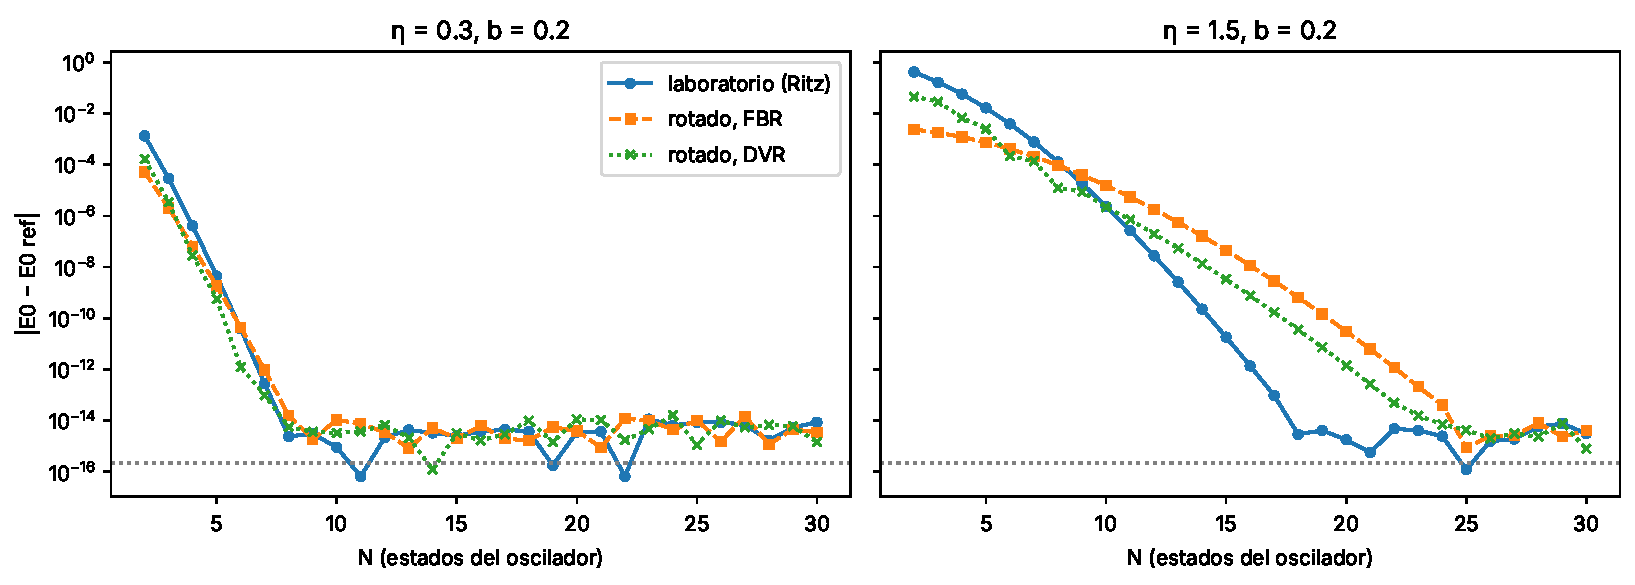
\includegraphics[width=\textwidth]{fig_convergencia.pdf}
\caption{Error of $E_0$ versus the number $N$ of oscillator states for the three discretizations, $b=0.2$. \todo{Pieza B.3: one or two sentences on the crossover.}}
\label{fig:conv}
\end{figure}

\section{Computable enclosures}\label{sec:cert}
Let $(\lambda_k,v_k)$, $k=0,1$, be the two lowest Ritz pairs of $PHP$, with $v_k=\sum_{n<N}\psi_n\otimes v_{k,n}$, and $r_k=Hv_k-\lambda_kv_k$.

\begin{lemma}[closed-form residual]\label{lem:res}
$\|r_k\|=\eta\sqrt{N/2}\,\|v_{k,N-1}\|$.
\end{lemma}
\begin{proof}\todo{Pieza C.1, in your own words.}\end{proof}

\begin{theorem}[Temple, Kato]\label{thm:kt}
Let $A$ be self-adjoint, let $(\alpha,\beta)$ contain exactly one eigenvalue $E$ of $A$, let $\|v\|=1$, $\lambda=\langle v,Av\rangle\in(\alpha,\beta)$ and $r=Av-\lambda v$. Then $\lambda-\|r\|^2/(\beta-\lambda)\le E\le\lambda+\|r\|^2/(\lambda-\alpha)$.
\end{theorem}
\begin{proof}\todo{Pieza C.2, in your own words. Cite \cite{temple1928,kato1949}.}\end{proof}

\begin{proposition}[a gap without spectral assumptions]\label{prop:gap}
Let $b<1$ and $\beta_2=\tfrac32-\tfrac{\eta^2}2-\tfrac b2$. Then $E_2\ge\beta_2$. If, moreover,
\begin{equation}\label{eq:checks}
\lambda_1-\|r_1\|>\lambda_0\qquad\text{and}\qquad\lambda_1+\|r_1\|<\beta_2,
\end{equation}
then $E_1\ge\beta_1:=\lambda_1-\|r_1\|$, and
\[
\lambda_0-\frac{\|r_0\|^2}{\beta_1-\lambda_0}\le E_0\le\lambda_0,\qquad
\lambda_1-\frac{\|r_1\|^2}{\beta_2-\lambda_1}\le E_1\le\lambda_1 .
\]
\end{proposition}
\begin{proof}\todo{Pieza C.3: Weyl's inequality applied to \eqref{eq:Hrot} with $\|W\|=b/2$ (cite a source for Weyl's inequality); the counting argument; then Theorem~\ref{thm:kt}.}\end{proof}

\begin{proposition}[enclosure of the Rabi matrix element]\label{prop:x}
Under \eqref{eq:checks}, let $\delta_0=\beta_1-\lambda_0$, $\delta_1=\min(\lambda_1-\lambda_0,\beta_2-\lambda_1)$, and assume $\|r_k\|<\delta_k$. Then
\[
\bigl|\,\xge-|\langle v_0,xv_1\rangle|\,\bigr|\le\sqrt2\left(\frac{\|r_0\|}{\delta_0}\sqrt{2\lambda_1+\eta^2+b}+\frac{\|r_1\|}{\delta_1}\,\|xv_0\|\right).
\]
\end{proposition}
\begin{proof}\todo{Pieza C.4: Davis--Kahan for one vector, the moment bound $H\ge\tfrac12x^2-\tfrac{\eta^2}2-\tfrac b2$, Cauchy--Schwarz.}\end{proof}

\begin{remark}
Every quantity in Propositions~\ref{prop:gap} and~\ref{prop:x} is computed from the $2N\times2N$ matrix $PHP$. The conditions \eqref{eq:checks} are \emph{verified}, not assumed: when they fail we increase $N$. \todo{Pieza C.5: the case $N=1$, $b=0$, where Theorem~\ref{thm:kt} is nearly attained. Say plainly that all computations are in floating point, so the enclosures are rigorous only up to rounding (interval arithmetic would remove this caveat).}
\end{remark}

\section{A certified validity map}\label{sec:map}
For each $(\eta,b)$ on a $46\times40$ logarithmic grid, $10^{-3}\le\eta\le2$, $0.005\le b\le0.9$, we take the smallest $N$ for which the enclosures of Propositions~\ref{prop:gap} and~\ref{prop:x} have relative width at most $10^{-6}$. We then bound the relative error of the first-order formulas.
\todo{Pieza C.6 and cell C4: the validation on 35 points (how many failures, largest $N$). Cell C5: read Fig.~\ref{fig:map} in words; give the two crossing values of $\eta$ for $\eta b$; the worst error of $\eta b e^{-\eta^2}$ for $b\le0.02$; the dark stripes in panel (b).}

\begin{figure}[h]\centering
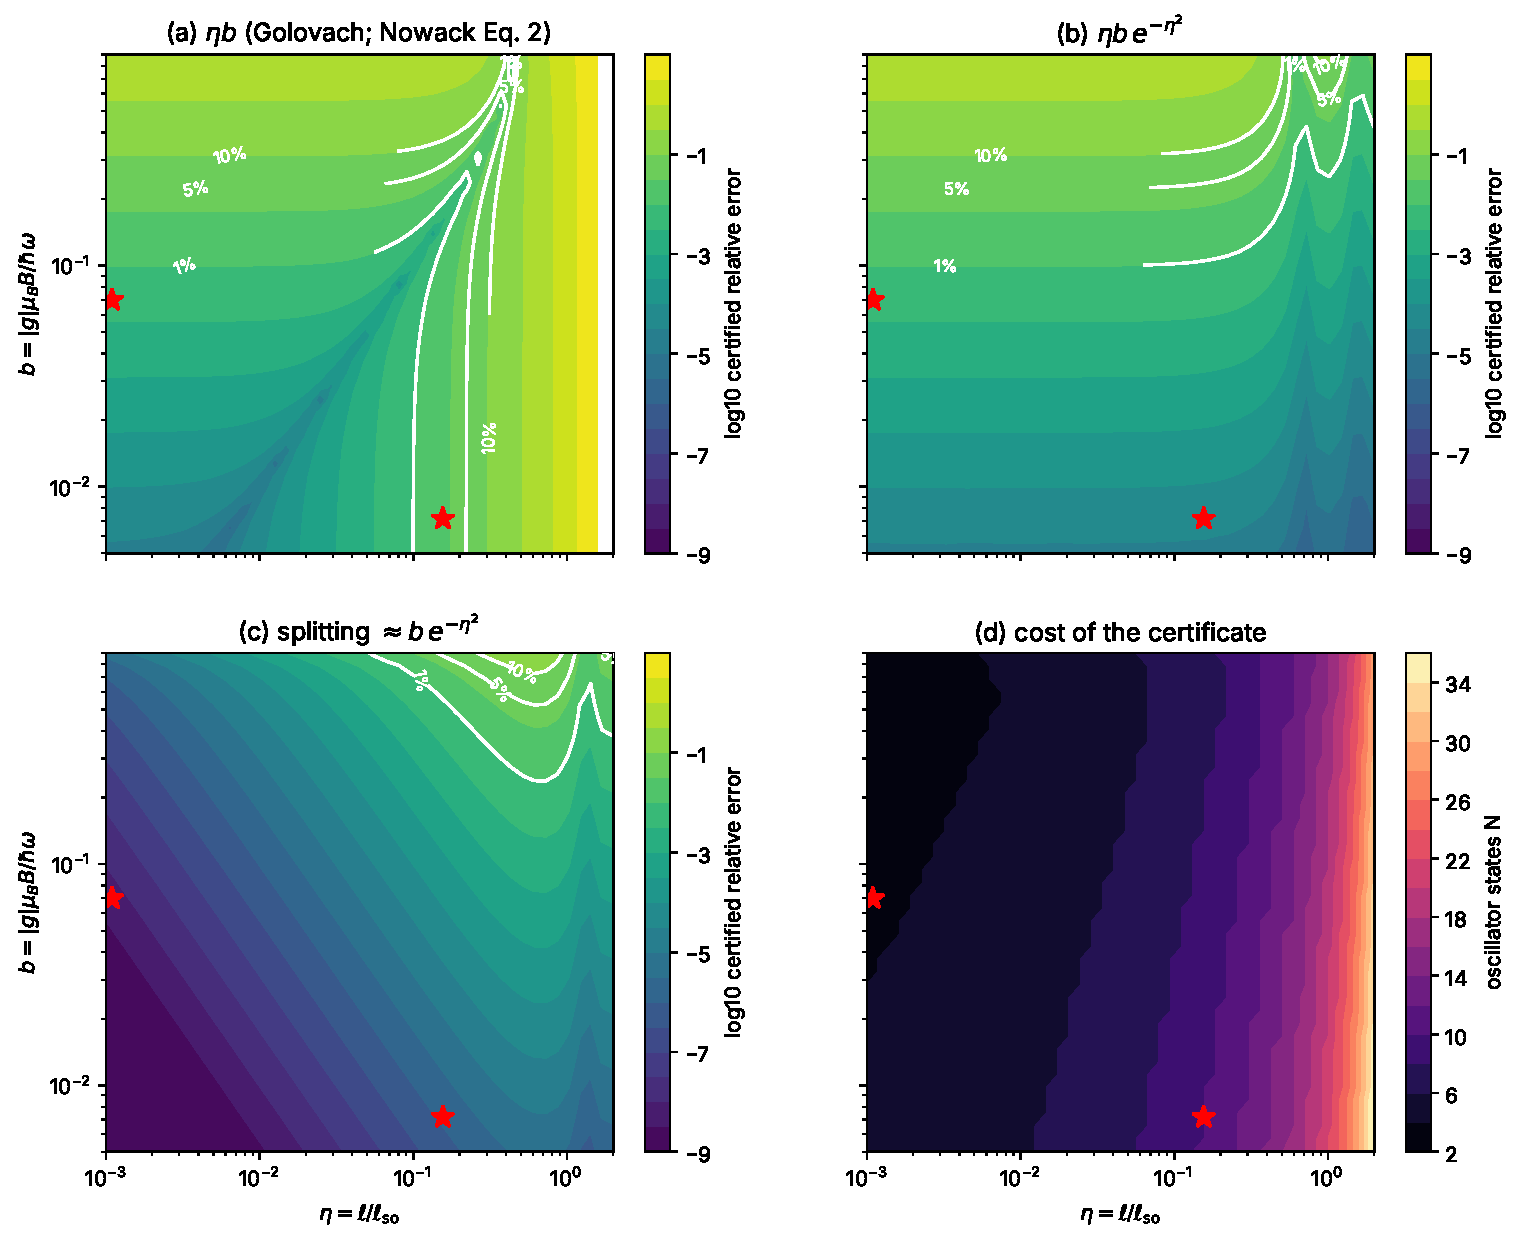
\includegraphics[width=\textwidth]{fig_mapa.pdf}
\caption{Certified relative error of (a) $\xge\approx\eta b$ \cite{golovach2006,nowack2007}, (b) $\xge\approx\eta be^{-\eta^2}$, (c) $E_1-E_0\approx be^{-\eta^2}$, and (d) the number of oscillator states used by the certificate. White contours: 1\%, 5\% and 10\%. Stars: the devices of Table~\ref{tab:devices}. \todo{Pieza C.6: finish the caption.}}
\label{fig:map}
\end{figure}

\begin{table}[h]\centering
\caption{Certified relative error of the first-order formulas for the two devices. \todo{Pieza C.6: fill from cell C5.}}
\begin{tabular}{lccc}\toprule
device & $\eta b$ & $\eta b\,e^{-\eta^2}$ & $N$\\\midrule
GaAs & & & \\
InAs & & & \\\bottomrule
\end{tabular}\end{table}

\section{What an energy-rewarded agent learns}\label{sec:agent}
\todo{Pieza C.6(b)--(c): an agent that chooses the discretization and $N$ to minimize $E_0+cN$ learns to prefer the DVR with few states, because the DVR undershoots. A learned fixed $N$ fails out of distribution, and its training used a reference that a real calculation does not have (the leak). The certified policy needs no reference. Connect, briefly and with citations, to reward hacking in machine learning for science.}

\begin{table}[h]\centering
\caption{Three policies, $b=0.2$, tolerance $10^{-6}$. \todo{Pieza C.6: fill from cell C6.}}
\begin{tabular}{lccc}\toprule
$\eta$ & energy-rewarded agent & certified $N$ & error, learned $N$\\\midrule
0.3 & & & \\
1.0 & & & \\
1.5 & & & \\\bottomrule
\end{tabular}\end{table}

\section{Related work}\label{sec:related}
\todo{Pieza D.1: EDSR theory \cite{rashbaefros2003,golovach2006,li2013}; experiments \cite{nowack2007,nadjperge2010}; DVR \cite{light1985,lombardi2004}; lower bounds and computer-assisted eigenvalue enclosures \cite{temple1928,kato1949,ronto2023} and one more source you find. How we differ, in one sentence each.}

\section{Limitations and outlook}\label{sec:limits}
\todo{Pieza D.3(b): at least four limitations (1D; Rashba only; floating point; $b<1$; mixed device parameters; GaAs needs no numerics; agents are exhaustive searches). Pieza E: strong spin--orbit systems \cite{froning2021} and whether a 1D Rashba model is adequate for holes.}

\section*{Data and code availability}
All numbers and figures come from the notebook \texttt{trabajo\_final\_espin.ipynb}, run top to bottom. The notebook, the device parameters and their sources are in the folder \texttt{trabajo-final-espin} of the repository
\url{https://github.com/cmorregof/methods_exam}. Physical constants: CODATA 2022 through \texttt{scipy.constants}.

\section*{Author contributions}
S.C.M.: formal analysis, investigation, software, writing (original draft). C.M.O.F.: conceptualization, methodology, supervision, writing (review and editing). \todo{adjust if needed}

\begin{thebibliography}{99}
\bibitem{rashbaefros2003} E. I. Rashba and Al. L. Efros, Orbital mechanisms of electron-spin manipulation by an electric field, \emph{Phys. Rev. Lett.} 91, 126405 (2003). doi:10.1103/PhysRevLett.91.126405
\bibitem{golovach2006} V. N. Golovach, M. Borhani and D. Loss, Electric-dipole-induced spin resonance in quantum dots, \emph{Phys. Rev. B} 74, 165319 (2006). doi:10.1103/PhysRevB.74.165319
\bibitem{nowack2007} K. C. Nowack, F. H. L. Koppens, Yu. V. Nazarov and L. M. K. Vandersypen, Coherent control of a single electron spin with electric fields, \emph{Science} 318, 1430 (2007). doi:10.1126/science.1148092
\bibitem{nadjperge2010} S. Nadj-Perge, S. M. Frolov, E. P. A. M. Bakkers and L. P. Kouwenhoven, Spin--orbit qubit in a semiconductor nanowire, \emph{Nature} 468, 1084--1087 (2010). doi:10.1038/nature09682
\bibitem{fasth2007} C. Fasth, A. Fuhrer, L. Samuelson, V. N. Golovach and D. Loss, Direct measurement of the spin-orbit interaction in a two-electron InAs nanowire quantum dot, \emph{Phys. Rev. Lett.} 98, 266801 (2007). doi:10.1103/PhysRevLett.98.266801
\bibitem{li2013} R. Li, J. Q. You, C. P. Sun and F. Nori, Controlling a nanowire spin-orbit qubit via electric-dipole spin resonance, \emph{Phys. Rev. Lett.} 111, 086805 (2013). doi:10.1103/PhysRevLett.111.086805
\bibitem{vurgaftman2001} I. Vurgaftman, J. R. Meyer and L. R. Ram-Mohan, Band parameters for III--V compound semiconductors and their alloys, \emph{J. Appl. Phys.} 89, 5815 (2001). \todo{add doi}
\bibitem{light1985} J. C. Light, I. P. Hamilton and J. V. Lill, Generalized discrete variable approximation in quantum mechanics, \emph{J. Chem. Phys.} 82, 1400 (1985). doi:10.1063/1.448462
\bibitem{lombardi2004} M. Lombardi, P. Barletta and A. Kievsky, Variational estimates using a discrete variable representation, \emph{Phys. Rev. A} 70, 032503 (2004). doi:10.1103/PhysRevA.70.032503
\bibitem{golubwelsch1969} G. H. Golub and J. H. Welsch, Calculation of Gauss quadrature rules, \emph{Math. Comp.} 23 (1969). doi:10.1090/S0025-5718-69-99647-1 \todo{add pages}
\bibitem{temple1928} G. Temple, The theory of Rayleigh's principle as applied to continuous systems, \emph{Proc. R. Soc. Lond. A} 119, 276 (1928). \todo{Pieza C: verify (taken from the reference list of \cite{ronto2023})}
\bibitem{kato1949} T. Kato, On the upper and lower bounds of eigenvalues, \emph{J. Phys. Soc. Jpn.} 4, 334 (1949). \todo{Pieza C: verify (taken from the reference list of \cite{ronto2023})}
\bibitem{ronto2023} M. Ronto, P. Jeszenszki, E. M\'atyus and E. Pollak, Lower bounds on par with upper bounds for few-electron atomic energies, arXiv:2301.02827 (2023). \todo{journal version?}
\bibitem{froning2021} F. N. M. Froning, L. C. Camenzind, O. A. H. van der Molen, A. Li, E. P. A. M. Bakkers, D. M. Zumb\"uhl and F. R. Braakman, Ultrafast hole spin qubit with gate-tunable spin--orbit switch, \emph{Nature Nanotechnology} (2021). doi:10.1038/s41565-020-00828-6 \todo{volume and pages}
\end{thebibliography}
\end{document}
